\documentclass[a4paper]{article}
\usepackage[a4paper,left=2cm,right=2cm,top=0.5cm,bottom=0.5cm,includehead,includefoot,headheight=0.1cm,heightrounded]{geometry}
\usepackage{amsmath}
\usepackage{amssymb}
\usepackage{graphics}
\usepackage{graphicx}
\usepackage[table,xcdraw]{xcolor}
\usepackage{float}
\usepackage{fontawesome}
\usepackage{ragged2e}
\usepackage{titlesec}
\usepackage{tikz}
\usepackage{pdfpages}
\usepackage{forest}
\usepackage[title]{appendix}
\usepackage[export]{adjustbox}
\usetikzlibrary{automata, positioning, shapes.symbols, arrows, chains, calc}
\usepackage[nottoc,numbib]{tocbibind}
\usepackage{shellesc}
\usepackage{minted}
\usepackage{listings}
\usepackage[hidelinks]{hyperref}
\usepackage[osfigures]{opensans}
\usepackage{lastpage}
\usepackage{fancyhdr}
\usepackage{mdframed}
\usepackage{bm}
\usepackage{array}
\usepackage{enumitem}
\usepackage[round]{natbib}
\usepackage{environ}
\usepackage{varwidth}
\usepackage{mathtools}
\usepackage{pagecolor}
\usepackage{wrapfig}
\usepackage{csquotes}
\usepackage[super]{nth}
\newlength{\MyMdframedWidthTweak}%
\NewEnviron{MyMdframed}[1][]{%
    \setlength{\MyMdframedWidthTweak}{\dimexpr%
        +\mdflength{innerleftmargin}
        +\mdflength{innerrightmargin}
        +\mdflength{leftmargin}
        +\mdflength{rightmargin}
    }%
    \savebox0{%
        \begin{varwidth}{\dimexpr\linewidth-\MyMdframedWidthTweak\relax}%
            \BODY
        \end{varwidth}%
    }%
    \begin{mdframed}[
        backgroundcolor=lightgrey,
        topline=true,
        rightline=false,
        leftline=false,
        linecolor=id7-aubergine,
        userdefinedwidth=\dimexpr\wd0+\MyMdframedWidthTweak\relax, 
        #1]
        \usebox0
    \end{mdframed}
}
\DeclarePairedDelimiter\abs{\lvert}{\rvert}%
\title{}
\author{}
\definecolor{infogreen}{rgb}{0.153, 0.682, 0.376}
\definecolor{id7-aubergine}{HTML}{5B3069}
\definecolor{id7-gray}{HTML}{3F4246}
\definecolor{body-text}{HTML}{333333}
\definecolor{id7-gold}{HTML}{886C11}
\definecolor{id7-burnt-orange}{HTML}{A14418}
\definecolor{id7-ruby-red}{HTML}{89102C}
\definecolor{id7-emerald-green}{HTML}{797906}
\definecolor{id7-sky-blue}{HTML}{204F79}
\definecolor{id7-sky-blue-accent}{HTML}{4d7294}
\definecolor{id7-sky-blue-tint}{HTML}{bccad7}
\definecolor{skyblue}{rgb}{0.125, 0.31, 0.475}
\setlength{\parindent}{0em}
\setlength{\parskip}{1em}
\definecolor{todocolor}{rgb}{0.688,0.8176,0.93137}
\newcommand{\todobox}[1] {\colorbox{todocolor}{\parbox{\textwidth}{\vspace{.75\baselineskip}\centering\parbox{0.95\textwidth}{\faicon{lightbulb-o} \textbf{TODO:} #1\vspace{.75\baselineskip}}}}}
\newcommand{\readbox}[1] {\colorbox{infogreen}{\parbox{\textwidth}{\vspace{.75\baselineskip}\centering\parbox{0.95\textwidth}{\textcolor{white}{\faicon{book} \textbf{#1}\vspace{.75\baselineskip}}}}}}
\def\labelitemi{\textcolor{id7-aubergine}{\textbullet}}
\def\labelitemii{\textcolor{id7-aubergine}{$\circ$}}
\def\labelitemiii{\textcolor{id7-aubergine}{--}}
\definecolor{infogreenlight}{rgb}{0.75,1,0.75}
\definecolor{termbg}{HTML}{232729}

\newcommand{\infobox}[1] {\colorbox{id7-sky-blue-tint}{\parbox{\textwidth}{\vspace{.75\baselineskip}\centering\parbox{0.95\textwidth}{\faicon{info-circle} \sffamily#1\vspace{.75\baselineskip}}}}}

\newcommand{\termbox}[1] {\colorbox{termbg}{\parbox{\textwidth}{\vspace{.75\baselineskip}\centering\parbox{0.95\textwidth}{ \sffamily#1\vspace{.75\baselineskip}}}}}

\newcommand{\boxedfigure}[2]{\begin{MyMdframed}\begin{figure}[H]
            \begin{center}\vspace{2em}\includegraphics[width=0.5\textwidth]{#1}\end{center}
            \caption{#2}
\end{figure}\end{MyMdframed}}

\newcommand{\widthboxedfigure}[3]{\begin{MyMdframed}\begin{figure}[H]
            \begin{center}\vspace{2em}\includegraphics[width=#3\textwidth]{#1}\end{center}
            \caption{#2}
\end{figure}\end{MyMdframed}}

\newcommand{\infoinlineicon}[1] {\colorbox{infogreenlight}{\faicon{info-circle} #1}}

\newcommand{\infoinline}[1] {\colorbox{infogreenlight}{#1}}

\definecolor{orange}{rgb}{0.9529,0.85176,0.5070588}

\newcommand{\warnbox}[1] {\colorbox{orange}{\parbox{\textwidth}{\vspace{.75\baselineskip}\centering\parbox{0.95\textwidth}{\faicon{exclamation-triangle} #1\vspace{.75\baselineskip}}}}}

\newcommand{\warninlineicon}[1] {\colorbox{orange}{\faicon{exclamation-triangle} #1}}

\newcommand{\warninline}[1] {\colorbox{orange}{#1}}

\titleformat{\section}
{\normalfont\sffamily\huge\color{id7-aubergine}}
{\thesection. }{0em}{}

\titleformat{\subsection}
{\normalfont\Large\sffamily\color{id7-aubergine}}
{\thesection}{0em}{}

\titleformat{\subsubsection}
{\normalfont\large\sffamily\color{id7-aubergine}}
{\thesection}{0em}{}
\fancyhf{}
\pagestyle{fancy}
\renewcommand{\headrulewidth}{0pt}
\lfoot{\textcolor{grey}{Adam Williams}}
\rfoot{\textcolor{grey}{Page \thepage{} of \pageref{LastPage}}}

\renewcommand*\footnoterule{\noindent\makebox[\textwidth]{
\includegraphics[width=\paperwidth]{divider}}}

\definecolor{grey}{rgb}{0.5,0.5,0.5}
\definecolor{lightgrey}{rgb}{0.96,0.96,0.96}

\def \spacedrule {\textcolor{id7-aubergine}{\hrule}\vspace{1em}}
\def \thedate {November \nth{15} 2018}
\lhead{\textcolor{grey}{\thedate}}
\rhead{\textcolor{grey}{Progress Report}}
% ======================

\begin{document}
    
\newgeometry{margin=0in}
\begin{titlepage}
    
    \tikz[remember picture,overlay] \node[opacity=1,inner sep=0pt] at (current page.center){
\includegraphics[width=\paperwidth,height=\paperheight]{bg_title_page}};
    \vspace{0.666\textheight} % height of the devil
    
    {\hspace{0pt}\vspace{0pt}\begin{tikzpicture}[scale=\paperwidth/1cm, overlay]
        \filldraw[draw=none,fill=white]
        (0, 0)
        -- (0.65838,0) 
        -- (0.71534285714,-0.1) 
        -- (0.7577,-0.0215)
        -- (0.8001, -0.1)
        -- (0.8571,0)
        -- (1, 0)
        -- (1, -0.45)
        -- (0, -0.45);

        \node[opacity=1,inner sep=0pt] at (0.7577, -0.15){
\includegraphics[width=6cm]{logotype}};
        \node[text width=15cm] at (0.39,-0.15) {\sffamily\fontsize{40}{10}\selectfont\textcolor{id7-aubergine}{Regular Expression\\\vspace{0.2cm}Refinement Types}};
        \end{tikzpicture}}
    
    {\par}
    \vspace{1.25cm}
    \vspace{3.5cm}
    {\hspace{0.75cm}\Huge \sffamily Progress Report}
    \vspace{0.16cm}
    {\par}
    {\hspace{0.75cm}\large \sffamily Adam Williams}
    
    \vspace{0cm}
    {\par}
    {\hspace{0.75cm}\large \sffamily Supervisor: Michael Gale}
    \vfill
\end{titlepage}
\restoregeometry
\restorepagecolor

\tableofcontents
\pagebreak[5]
    
    \section{Introduction}
    
    Within type systems, refinement types allow for predicate-based constraints to be applied to type definitions in order to restrict the domain of elements which belong to the type.
    
    For example, a local variable used to store natural numbers could be constrained via $\{n: \mathbb{N}\ \mid n \leq 5\}$. Only $\{0, 1, 2, 3, 4, 5\}$ would be permitted for values of $n$ under this refinement type.
    
    This project applies refinement types to strings which enforce membership of $L(R)$ for some regular expression $R$. For example, $\{s: \Sigma^* \mid s \in L(ab+)\}$ \footnote{For some regular expression $R$, $L(R)$ is used to denote the language that it accepts} would allow \texttt{"ab"} to be assigned as a value of some variable $s$, but not \texttt{"a"}. This is motivated by the common use of regular expressions as a validation mechanism to provide security in systems that handle user input, with the ultimate aim of eliminating potential vulnerabilities at compile time.
    
    Designing a proof-of-concept language with syntax for expressing such refinement types and implementing a type checker allows for the feasibility of such compile-time checks to be evaluated.

    Per the specification included in Appendix \ref{spec}, Weeks 1-9 of the project were scheduled to involve implementing and testing a prototype parser and type checker for the language.
    
    \section{Project State}
    
    Early on in the project lifetime it was decided to begin work on a phase 1 prototype with a simplified goal to gain some experience working with refinement types and type checkers in general. Once complete, work would continue in a 2nd phase which introduced regular expressions.
    
    The project is currently ahead of schedule. By week 7, both phases 1 and 2 have been completed to a satisfactory standard.
    
    \subsection*{Phase 1}
    
    Prototype work began with simple refinement types which could be applied to natural numbers. The final syntax was similar to the example presented in the specification:
    
    \begin{minted}{javascript}
function Main(id: uint): uint[< 4] {
    // A simple function declaration, returns an int less than 4
    return 0
}
function StackOne(): uint[> 5] {
    // This function must return an unsigned int greater than 5
    return LookupUserById(1)
}
    \end{minted}
    
    As the \texttt{Main()} function returns an integer less than 4, a violation is present within \texttt{StackOne()} where it is returned. This violation arises because \texttt{StackOne}'s return type is constrained to be greater than 5.
    
    Running this simple program with the prototype tool yields the following output:
    

    \termbox{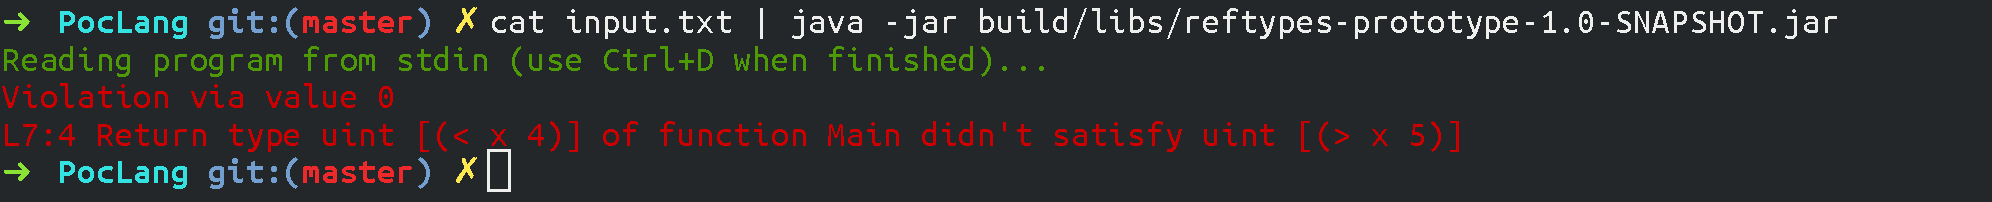
\includegraphics[width=\linewidth]{term1}}
    
    The prototype tool has found a valid value (here, $0$) which satisfies $x < 4$ but violates $x > 5$. If integrated into a ``real'' programming language, this would be identified at compile time and prevent successful compilation.
    
    This initial version of the prototype which operated exclusively on the natural numbers was built using the following tools, libraries and languages:
    
    \begin{description}
        \item[JavaSMT] Library which provides an abstraction layer over a variety of different SMT solvers (such as Z3 and MathSAT) and provides added type safety \citep{karpenkov2016javasmt}.
        \item[ANTLR 4] An $LL(*)$ lexer and parser generator which can target languages such as Java, Go and C\# \citep{parr2011ll}. In the initial prototype, ANTLR was used to generate a combined lexer-parser using a composite grammar in which both non-terminals and terminal symbols (tokens) are specified.
        \item[JUnit] A unit testing framework for Java. Used to build a collection of unit and integration tests to support refactoring and a test-driven development approach.
        \item[Gradle] Industry-standard build automation system which co-ordinates the grammar generation, Java class compilation, construction of a JAR file with shaded dependencies and running the unit tests.
        \item[IntelliJ IDEA] An advanced Java IDE with leading code inspection and analysis capabilities \citep{ideainspections} \citep{Jemerov:2008:IRI:1636642.1636655}. Used in conjunction with the official ANTLR plugin which provides grammar syntax highlighting and analysis.
    \end{description}

    The general steps involved in the process are described below.
    
    \tikzstyle{line} = [draw, -latex']
    \tikzset{arrow/.style={
            minimum height=1.2cm,%
            inner sep=1em,
            shape=signal,
            signal from=west,
            signal to=east,
            signal pointer angle=110,
            text depth=.25ex,
            text height=1.5ex,
            fill=skyblue,
            baseline,
            text centered, text=white
    }}
    \tikzset{arrowcur/.style={
            fill=id7-sky-blue-accent
    }}
    \begin{figure}[H]
            \begin{tikzpicture}[node distance=-\pgflinewidth, auto]
            \sffamily{
                \begin{scope}[start chain=transition going right,node distance=-\pgflinewidth]
                \node [arrow, arrowcur, on chain] {\faCogs{} \textbf{Parsing}};
                \node [arrow, on chain] {\faSearch{} Initial walk};
                
                \node [arrow, on chain] {\faCheckCircle{} Type checking};
                \node [arrow, on chain] {\faFileText{} Reporting};
                \end{scope}
            }
            \end{tikzpicture}
    \end{figure}
    

    In the \textbf{Parsing} step, the ANTLR parser is used to generate a parse tree from the input program. For example, consider the following simple function declaration:
    
    \begin{minted}{javascript}
function Main(id: uint[> 1]): uint {
    return 1*1
}
    \end{minted}
The parse tree generated for this function definition is shown in figure \ref{tree}.

\begin{figure}[H]
\begin{forest}
[program
[function
[function\_sig
[function]
[ ]
[Main]
[(]
[argument\_decl
[id]
[:]
[ ]
[type
[type\_keyword
[uint]
]
[{[}]
[int\_constraint
[>]
[ ]
[1]
]
[{]}]
]
]
[)]
[:]
[ ]
[type
[type\_keyword
[uint]
]
]
[ ]
[\{]
[\textbackslash{}n]
]
[body
[body\_line
[return\_stmt
[return]
[ ]
[expr
[expr
[value\_ref
[1]
]
]
[*]
[expr
[value\_ref
[1]
]
]
]
]
]
[\textbackslash{}n]
]
[\}]
]
[<EOF>]
]]
\end{forest}
\caption{Parse tree for the \texttt{Main} function. Note that the \texttt{type} non-terminal describes everything about the types, including any applicable constraints. \label{tree}}
\end{figure}
    
    For the phase 1 prototype, the lexer and parser are both generated from the same grammar file. Any \emph{syntactical} errors are found during this step, these must be fixed before the type checking will be carried out.
    
    \begin{figure}[H]
        \begin{tikzpicture}[node distance=-\pgflinewidth, auto]
        \sffamily{
            \begin{scope}[start chain=transition going right,node distance=-\pgflinewidth]
            \node [arrow, on chain] {\faCogs{} Parsing};
            \node [arrow, arrowcur, on chain] {\faSearch{} \textbf{Initial walk}};
            
            \node [arrow, on chain] {\faCheckCircle{} Type checking};
            \node [arrow, on chain] {\faFileText{} Reporting};
            \end{scope}
        }
        \end{tikzpicture}
    \end{figure}

    The language designed for this prototype allows for functions to be called from within functions that may occur anywhere within the program code. As a result, it is necessary to perform one initial pass through the parse tree in order to collect function names to store in the function table. This table stores the identifier (\texttt{Main} in the example used previously) and the return type.
    
    ANTLR provides a \texttt{BaseListener} class which can be extended in order to create a listener which is called for each non-terminal encountered when walking the parse tree.
    
    The proof-of-concept language implementation uses one listener which is parametrised with a \texttt{VisitorPhase} value to specify the stage at which the listener should operate. This is set to \texttt{COLLECTING\_FUNCTIONS} for the \textbf{Initial walk} stage.
    
    It is within this stage that function re-declarations can be discovered and reported. Errors are stored centrally and associated with the input token closest to the origin of the problem.
    
    \widthboxedfigure{FunctionTable.png}{Dependency diagram showing how the functions declarations are stored and the data stored alongside them.}{0.5}
    
    \begin{figure}[H]
        \begin{tikzpicture}[node distance=-\pgflinewidth, auto]
        \sffamily{
            \begin{scope}[start chain=transition going right,node distance=-\pgflinewidth]
            \node [arrow, on chain] {\faCogs{} Parsing};
            \node [arrow, on chain] {\faSearch{} Initial walk};
            
            \node [arrow, arrowcur, on chain] {\faCheckCircle{} \textbf{Type checking}};
            \node [arrow, on chain] {\faFileText{} Reporting};
            \end{scope}
        }
        \end{tikzpicture}
    \end{figure}

    Once the function definitions have been collected, the main type checking phase can begin. This covers validating function calls, variable assignments and return statements.
    
    This is mainly achieved by visiting function bodies and initialising a stack for scoped storage of local variables and function arguments as is standard in most programming languages \citep[p. 88]{watt2004programming}.
    
    For types with a provided constraint, the JavaSMT library is used to check the inverted \emph{expected} type against the \emph{actual} type.
    
    For example, consider the code below:
    
    \begin{minted}{javascript}
    function Main(): uint[> 4] {
        var u: uint[< 10]
        return u
    }
    \end{minted}
    
    In this case, the return value of \texttt{Main} is constrained as $\{x: \mathbb{N} \mid{} x > 4\}$. When the \texttt{return u} statement is checked, the \emph{expected} type is $\{x: \mathbb{N} \mid{} x > 4\}$ and the \emph{actual} type is $\{x: \mathbb{N} \mid{} x < 10\}$. The \emph{expected} type is negated to give $\{x: \mathbb{N} \mid{} x \le 4\}$ and this constraint, along with the constraint defined by the \emph{actual} type are passed to the SMT solver to find a model. This model will include a value for $x$ that satisfies the conjunction of the two constraints.
    
    If the SMT theorem is satisfiable, we have found a violation -- it is possible for the refinement type constraints to not hold during execution. These are reported via the central error reporting mechanism.
    
    \begin{figure}[H]
        \begin{tikzpicture}[node distance=-\pgflinewidth, auto]
        \sffamily{
            \begin{scope}[start chain=transition going right,node distance=-\pgflinewidth]
            \node [arrow, on chain] {\faCogs{} Parsing};
            \node [arrow, on chain] {\faSearch{} Initial walk};
            
            \node [arrow, on chain] {\faCheckCircle{} Type checking};
            \node [arrow, arrowcur, on chain] {\faFileText{} \textbf{Reporting}};
            \end{scope}
        }
        \end{tikzpicture}
    \end{figure}

    During the 4th and final step of execution, the prototype application reports the errors discovered previously. Each of these includes a line number and message to describe the problem.
    
    These are simply printed to the standard error stream at the command line, but a real language could show these violations in an IDE to highlight problems inline.

\subsection*{Phase 2}

Once unsigned integer constraints were complete and a set of passing test cases had been written, the focus shifted to adding \texttt{string} support. A new type keyword was added, and the grammar was modified to accept regular expression constraints as shown in the example below.

\begin{minted}{javascript}
function LookupUserById(): string[/g+/] {
    return "f"
}
\end{minted}

Adding support for these constraints required being able to parse regular expressions. This was more challenging than anticipated -- although BNF descriptions of regular expressions are readily available, they are indirectly left-recursive. ANTLR, along with all $LL$ parser generators, requires that such production rules are removed before a working parser can be generated \citep{dick1990parsing}.

It is reasonably straightforward to remove left-recursion by introducing new production rules, however another issue arised with the programming language grammar's tokens:

\begin{minted}{antlr}
IDENTIFIER : [A-Za-z_] [A-Za-z_0-9]* ;
CHARACTER  : ~('\n'|'\r'|'.'|'('|')'|'['|']'|'*'|'+'|'/'|'|') | ESCAPED_META;
\end{minted}

The \texttt{IDENTIFIER} token was used for function and variable names. The \texttt{CHARACTER} token was used for single characters within a regular expression. As the two token definitions overlapped, only one would be identified by the lexer which had the effect of breaking the parsing of either the regular expressions, or the function definitions.

The fix for this issue was to use lexical modes. When the start of a string constraint is detected, the lexer should switch into a \texttt{REGEX} mode and match arbitrary characters with the \texttt{CHARACTER} token. At the end of the regular expression the mode should return to the default. Unfortunately, lexical modes are not supported in ANTLR's composite grammars and it was therefore necessary to split the parser and lexer into separate grammar files.


\begin{figure}[H]
    \begin{center}
    \begin{forest}
[re
  [simple\_re
    [basic\_re
      [plus
        [elementary\_re
          [range
            [positive\_range
              [{[}]
[range\_items
                [range\_item
                  [lax\_character
                    [A]
                    ]
[-]
[lax\_character
                    [Z]
                    ]
                  ]
                ]
[{]}]
              ]
            ]
          ]
[+]
        ]
      ]
[concat\_prime
      [simple\_re
        [basic\_re
          [elementary\_re
            [character
              [a]
              ]
            ]
          ]
[concat\_prime]
        ]
      ]
    ]
[union\_prime]
  ]
[/]
]
[{]}]
]]
    \end{forest}
    \end{center}
    \caption{\label{regextree}Parse tree for regular expression \texttt{[A-Z]+}.}
\end{figure}

Once this parsing was complete, it should have simply been a matter of taking advantage of the SMT solver's regular language membership support to find violations in much the same way as was performed on the integers. String (and regular expression support) is not universal amongst SMT solvers, however -- and JavaSMT did not provide an abstraction layer over such functionality.

As a result, the decision was made to build Z3 from source and use its Java bindings instead of the JavaSMT library. Z3 includes Z3str3 which is able to efficiently support solving string equations and predicates involving regular language membership \citep{berzish2017z3str3}. The original code which used the JavaSMT APIs to solve constraint problems with integers was then modified to use Z3. An adapter was written to construct a Z3 regular expression object from a parse tree.

The final prototype allows us to write a program like the one below:

\begin{minted}{javascript}
function SecondaryFunction(): string[/g+|f+/] {
    return "f"
}
function Main(): string[/f+/] {
    return SecondaryFunction()
}
\end{minted}

It will correctly determine that the union of \texttt{g+} in the constraint of \texttt{SecondaryFunction}'s return type is incompatible with \texttt{Main}'s return type:

\termbox{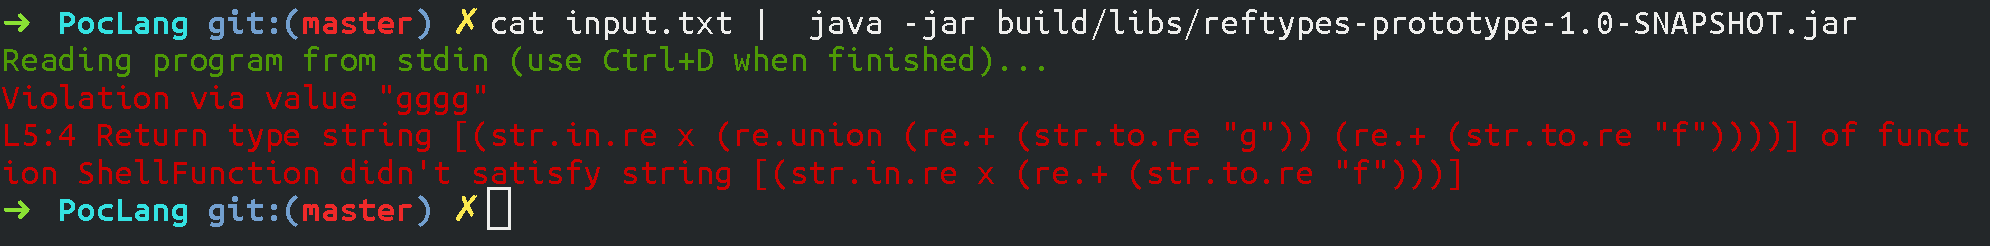
\includegraphics[width=\linewidth]{term2}}

\section*{Project Management}

The following objectives were described in the project specification (Appendix \ref{spec}):

\begin{enumerate}
    \item Formalise a type system that supports types predicated with a regular expression pattern that elements of the refined type will satisfy (be matched by).
    \begin{enumerate}
        \item Explore the consequences of typical string operations (e.g. concatenation) and define the type of
        their return value when applied to elements of the regular expression type.

        \item At minimum, this should allow for simple functions to be declared that can safely accept/return a
        particular regular expression input.
        \item Evaluate the rate of false positives when compared to existing static analysis
    \end{enumerate}
    \item Implement such a type system that can guarantee type safety, built against a simplified proof-of-concept
    language.
    \begin{enumerate}
        \item Test the implementation against a variety of test cases. The testing strategy should make use of
        automated unit tests, and manual system testing considering both general expected input as well as
        any relevant ``edge-cases'' that need to be handled.
    \end{enumerate}
\end{enumerate}

Objective 2 and the sub-objective related to testing has been completed as of the time of writing. 26 individual passing JUnit test methods have been defined which cover the broad areas described below:

\begin{description}
    \item[Parsing] Tests for simple syntactically valid and invalid programs, as well as parser regression tests for functions that were incorrectly parsed during development and subsequently fixed.
    \item[Simple type checks] Such as returning a string from a function marked as returning a string.
    \item[Other checks] Including function/variable re-declaration.
    \item[Integer refinement types] As described above, constraint violations for integer inequalities.
    \item[Regexp refinement types] As described above, constraint violations for regular language membership.
\end{description}

\termbox{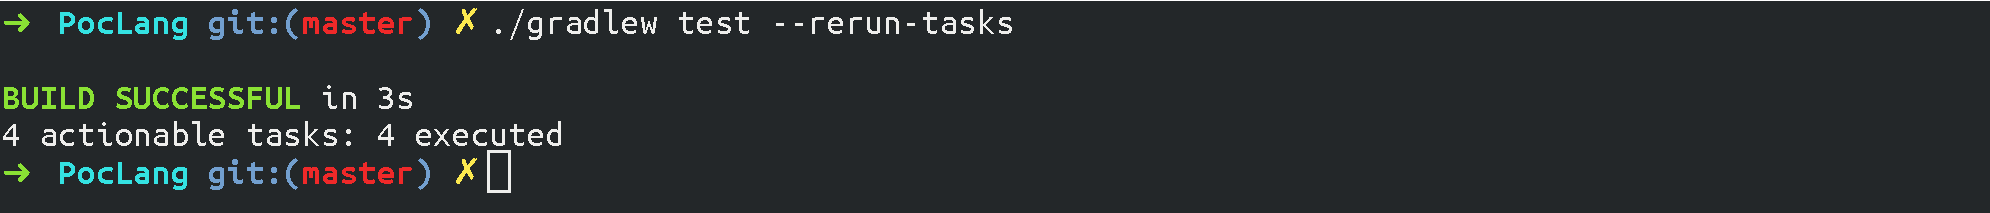
\includegraphics[width=\linewidth]{term3}}

Manual testing has taken place throughout and has been used to influence development of new unit tests.

Objective 1. (b) has been completed, in addition to local variable type constraints. Objectives 1. (a)\footnote{It should be reasonably trivial to define the plus operation for strings and infer the type constraint to be the concatenation of all involved regular expressions.} and (c) have not yet been completed.

This level of progress is in line with the original schedule, which allocated false positive rate evaluation to occur in early February of 2019 (with implementation to be finished in late November and testing to take place from December until January).

Immediate next steps once these objectives are complete will involve making the prototype language more expressive by introducing constructs to control execution flow. If time permits, the \emph{stretch objectives} will also be considered. There does not appear to be a need to make changes to the schedule at this time.

Throughout the project lifetime, code has been managed using the Git version control system. This has proved an invaluable tool for managing and syncing project assets and code.

\pagebreak[5]

\section{Conclusion}

In conclusion, development has proceeded reasonably well. There were some setbacks -- parsing challenges as well as needing to replace the SMT solver library which required refactoring time -- but the end result is a working prototype which implements refinement types for both integer inequalities and regular language membership.

Most of the objectives for the project have been met, including some which were scheduled to be completed later in the project's life. As a result, the project is on track for completion.

\bibliographystyle{agsm}
\bibliography{references}

\begin{appendices}
\titleformat{\section}
{\normalfont\sffamily\huge\color{id7-aubergine}}
{Appendix \thesection{} -- }{0em}{}
\section{Specification}

The original specification as submitted at the start of Term 1 is included overleaf.
\label{spec}
\end{appendices}
\includepdf[pages=2-]{../specification/spec.pdf}


\end{document}
